\documentclass[tikz,border=2pt]{standalone}
\usepackage{tikz}
\usetikzlibrary{arrows.meta,positioning}
\begin{document}
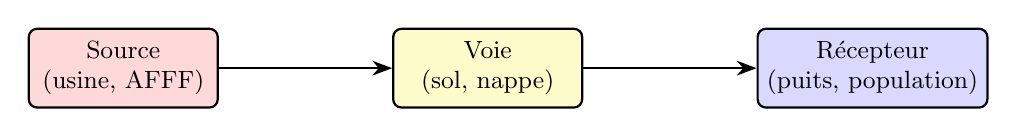
\begin{tikzpicture}[
    font=\small,
    >=Stealth,
    box/.style={draw, thick, rounded corners=3pt, align=center, minimum width=2.4cm, minimum height=1cm}
]
\node[box, fill=red!15] (s) {Source\\ (usine, AFFF)};
\node[box, fill=yellow!20, right=2.2cm of s] (v) {Voie\\ (sol, nappe)};
\node[box, fill=blue!15, right=2.2cm of v] (r) {R\'ecepteur\\ (puits, population)};
\draw[thick, -{Stealth[length=2.5mm]}] (s) -- (v);
\draw[thick, -{Stealth[length=2.5mm]}] (v) -- (r);
\end{tikzpicture}
\end{document}
